\chapter{ Aprendizaje Automático }
Aprendizaje Automático o \textit{Machine Learning} es una rama de la inteligencia artificial, el cual construye un modelo matemático basado en datos de muestra, conocidos como datos de entrenamiento, de forma a realizar predicciones o tomar decisiones sin que haya sido programado de forma explícita para realizar dicha tarea.\cite{zhang2020matrix}

Una definición más orientada a la ingeniería podría ser:

Se dice que un programa de computadoras aprende de una experiencia E respecto a una tarea T y alguna forma de medida de rendimiento P, si el rendimiento en la tarea T, medido por P, mejora con la experiencia E.\cite{mitchell1997machine}

Para entender un poco mejor utilicemos un ejemplo de un programa de aprendizaje automático, como podría ser un filtro de spam de correos electrónicos. Este filtro de spam puede aprender a detectar y marcar los correos mediante ejemplos proveídos por los usuarios, tanto de aquellos correos que el usuario marcó como un spam, así como de correos que el usuario considera que no lo son. Estos datos de ejemplo que el programa puede utilizar para aprender de ellos son llamados conjuntos de entrenamiento.

Para este caso la tarea T es la de marcar nuevos correos electrónicos como spam, la experiencia E es el entrenamiento con los datos, y la medida del rendimiento P podría ser la proporción de acierto o \textit{Accuracy} de los correos correctamente clasificados como spam o no.

\section{Tipos de sistemas de aprendizaje automático}
Los sistemas de aprendizaje automático pueden clasificarse de acuerdo a la cantidad y el tipo de supervisión que necesitan durante la fase de entrenamiento. Existen 3 grandes categorías de las cuales hablaremos a continuación:

\begin{itemize}
    \item Aprendizaje supervisado: En este tipo de aprendizaje, el conjunto de entrenamiento que se provee al programa incluye las soluciones deseadas, a estas soluciones se les conoce como etiquetas o \textit{labels}. Este método aprende una regla general la cual mapea el conjunto de entradas con las salidas deseadas.
    En el aprendizaje supervisado podemos dividir las tareas en dos enfoques principales, la Clasificación y Predicción de un valor numérico generalmente realizado por medio de la Regresión. 

    \begin{itemize}
        \item Clasificación: Consiste en brindar ejemplos de entradas indicando a que clase o clases pertenece, de forma a poder realizar el entrenamiento y de esa forma para nuevas entradas poder clasificar dentro de alguna de las clases contempladas.
        \item Predicción: Consiste en brindar datos de entrada con un conjunto de características y un valor objetivo, de forma que con el entrenamiento para las nuevas entradas es posible predecir el valor objetivo a partir del conjunto de características. Este tipo de tareas se lo conoce como Regresión.
    \end{itemize}
    \item Aprendizaje No-supervisado: En este tipo de  aprendizaje, el conjunto de entrenamiento que se provee al programa no incluye las soluciones deseadas o conocidas. La principal tarea de este método es la de encontrar soluciones por si mismo (por ejemplo, patrones o estructuras en los datos).
    \item Aprendizaje por refuerzo: Al tipo de aprendizaje basado en la retroalimentación se lo conoce como aprendizaje por refuerzo. En este método los datos de entrenamiento son proveídos en forma de recompensas (positivas o negativas) por medio de la retroalimentación a un agente de inteligencia artificial que interactúa con un entorno dinámico. La retroalimentación entre sistema de aprendizaje y la experiencia obtenida por el agente es muy útil para mejorar el rendimiento en la tarea que está aprendiendo.
\end{itemize}

\section{Redes Neuronales Artificiales}
Las redes neuronales artificiales son algoritmos bio-inspirados, es decir, están vagamente inspirados en el cerebro biológico. Como ocurre en el cerebro, las redes neuronales artificiales consisten en unidades simples llamadas neuronas las cuales se encuentran interconectadas entre si. Estas reciben, procesan y transmiten señales a otras neuronas actuando como un interruptor.

Los elementos de una red neuronal son bastantes simples, la complejidad y el poder de estos sistemas proviene de la interacción entre sus elementos. Por ejemplo, el cerebro humano cuenta  con más de cien mil millones de neuronas y cien billones de conexiones.

\subsection{Perceptrón}
El concepto de perceptrón se encuentra inspirado en las neuronas biológicas, cuya tarea principal es la de bloquear o dejar pasar las señales. Las neuronas reciben estas señales eléctricas, si la señal sobrepasa cierto umbral, la neurona lanza una señal de salida. \\
\begin{figure}[H]
    \centering
    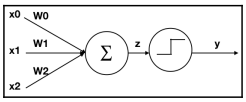
\includegraphics{capitulos/img/perceptron.png}
    \caption{Comportamiento del perceptrón}
    \label{fig:perceptron}
\end{figure}
Un perceptrón busca imitar ese mismo comportamiento, de la manera en la que se muestra en la figura \ref{fig:perceptron}. El mismo puede recibir múltiples datos de entrada \(X = {x_{0},x_{1},x_{2},...,x_{n}}\), entonces estos datos son multiplicados por un conjunto de pesos \(W = {w_{0},w_{1},w_{2},...,w_{n}}\). La suma ponderada z de estos datos de entrada, pasa por una función de activación, devolviendo así un valor y dependiendo del tipo de función de activación. También es posible expresarlo matemáticamente por medio de la siguiente fórmula: 
\begin{equation}
z = \sum_{i=1}^{n} w_{i} x_{i} = w^{T}x
\end{equation}
Este es el modelo matemático de una neurona, representado como una suma explícita y como una operación matricial. El término \(w^{T}x\)  es la representación vectorizada de la fórmula, donde \textit{w} es el peso de la matriz que primeramente es transpuesta y luego es multiplicada por un vector de entradas \textit{x}. Para obtener una descripción matemática completa podríamos añadir una constante \textit{b}, llamado bias.
\begin{equation}
z = \sum_{i=1}^{n} w_{i} x_{i} + b = w^{T}x + b
\end{equation}
Con esto obtenemos una expresión genérica de una ecuación lineal, el cual es  todo el proceso previo a su paso por la función de activación, la cual determinara si el perceptrón deja pasar la señal.
Existen muchas variantes para la función de activación, La función de activación mas sencilla es la función de paso. La salida de la neurona será aproximada por esta función, la cual se expresa por medio de la siguiente ecuación:
\begin{equation}
f(x)=\left\lbrace\begin{array}{c} 1~~~si~ (w^{t} x+b) > 0 \\ 0~~~caso~contrario~~ \end{array}\right.
\end{equation}

\subsection{Funciones de activación}
Existen varios tipos de funciones de activación, donde dependiendo de la tarea o valor buscado, estas pueden ser más o menos útiles. A su vez, estas funciones usualmente son utilizadas para agregar la no-linealidad, ya que sin esto solo podríamos tener soluciones lineales. Algunas de las funciones de activación más utilizadas son la sigmoide, tanh y la relu (\textit{rectified linear unit}) los cuales se muestran en la figura \ref{fig:funcionesActivacion}
\begin{figure}[h!]
    \centering
    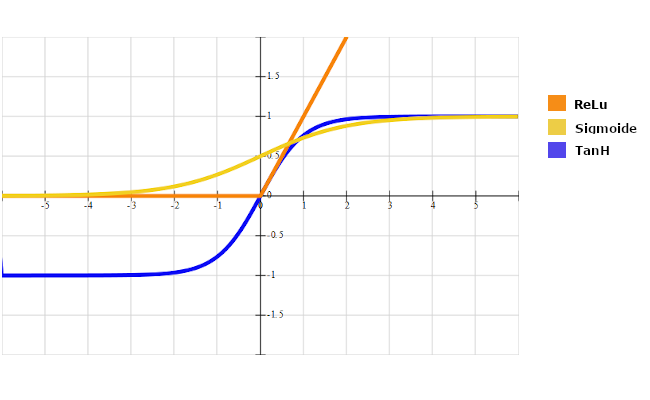
\includegraphics[width=1\textwidth]{capitulos/img/funcion_activacion.png}
    \caption{Funciones de Activación}
    \label{fig:funcionesActivacion}
\end{figure}
\newpage
\subsection{Arquitectura y aprendizaje}
Si muchas neuronas son conectadas entre sí, una red neuronal artificial es creada. En general, toda neurona de la red neuronal artificial está asociada a una capa. Cada neurona está conectada a todas las neuronas de la capa anterior y de la siguiente. Estas conexiones están ponderadas por un peso.\\
Un ejemplo de una arquitectura de redes neuronales artificiales se puede observar en la figura \ref{fig:redNeuronal}, donde se encuentra divida en tres áreas. La primera área contiene a la capa de entrada, y es la encargada de recibir y alimentar a la red con los datos de entrada. El área intermedia está conformada por una o más capas y son conocidas como capas ocultas, donde el número de capas ocultas determina la profundidad de la red. Por último, la última área contiene a la capa de salida que dependiendo de la tarea puede tener uno o más neuronas de acuerdo a los posibles valores de salida.\\
\begin{figure}[H]
    \centering
    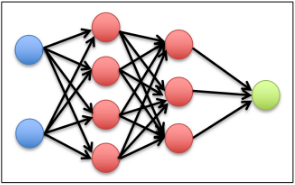
\includegraphics{capitulos/img/redNeuronal.png}
    \caption{Ejemplo de red neuronal}
    \label{fig:redNeuronal}
\end{figure}
Una vez que el peso de cada una de las conexiones de la red es establecido, es posible calcular un valor de salida para cada entrada de la red neuronal. En la mayoría de los casos, los pesos son establecidos de manera aleatoria por lo que los valores de salida calculados pueden ser diferentes a lo esperado. La idea es ajustar estos pesos de manera individual de forma a que el error cuadrático medio entre los valores calculados y los valores esperados sean mínimos, esto se realiza por medio del método de retropropagación o \textit{backpropagation}.\\

Primeramente, se calcula el resultado para un registro del conjunto de datos conocido, luego se calcula el error entre el resultado calculado y el resultado esperado. El error es propagado hacia atrás, pasando por todas las capas, empezando por la última capa y terminando con los pesos individuales de la primera capa de la red neuronal. La distribución del error toma lugar como una función de los valores de los pesos individuales. Una vez que los pesos individuales son cambiados, se procede a realizar el mismo procedimiento con un nuevo registro del conjunto de datos.\\

Para minimizar el error, se utiliza el método de descenso del gradiente, el cual al igual que el algoritmo de retropropagación son explicados en detalle en \cite{rashid2016make}.\\

Por otro lado tenemos el ratio de aprendizaje o \textit{Learning Rate} el cual es un indicador de cuánto cambian los pesos en cada iteración, Un valor de \textit{Learning rate} alto nos acerca de forma más rápida al error mínimo, pero una valor más bajo puede converger mejor. En la mayoría de los casos los valores elegidos son de 0.001 a 0.3.\\

Generalmente el entrenamiento de una red neuronal artificial con un solo conjunto de datos no es suficiente para alcanzar el mínimo error de salida, esto especialmente para valores bajos de \textit{Learning Rate}. Para mejorar esto, se realizan varias pasadas del conjunto de datos completo a través de la red neuronal, a cada pasada se lo conoce como época o \textit{epoch}. 

\section{Aplicación de Machine Learning en Redes Ópticas Elásticas}

En esta sección presentamos un estudio bibliográfico  del estado del arte de algunas técnicas de \textit{Machine Learning} aplicadas a problemas existentes en redes ópticas elásticas.

Panchali Datta Choudhury y Tanmay De, nos presentan un analisis del estado del arte  del uso de técnicas de \textit{Machine Learning} en redes ópticas elásticas \cite{choudhury2019recent}.

Algunas de las áreas presentadas por los autores en donde actualmente se utilizan estas técnicas son las siguientes:



\begin{itemize}
    \item Evaluación o predicción de la calidad de servicio
    
    Investigaciones como la propuesta en \cite{panayiotou2019data}, presenta un modelo de asignación de ancho de banda en EON teniendo en consideración los requisitos de la calidad del servicio o \textit{Quality of Service} (QoS) de la red. Utilizando la técnica de Aprendizaje Reforzado o \textit{Reinforcement Learning} para resolver el problema de asignación de ancho de banda, donde la función de recompensa para el modelo de aprendizaje reforzado se basa en el cumplimiento o no de los requisitos de QoS.
    
    \item Supervivencia
    
    Se hace uso del aprendizaje por refuerzo profundo en el trabajo \cite{luo2019leveraging}, explorando el problema de optimización de una red en general teniendo en cuenta la capacidad de supervivencia de la misma. Para ello se utilizó un enfoque de aprendizaje por refuerzo profundo, utilizando dos agentes, en donde uno de ellos se utiliza para proporcionar un esquema de trabajo y el otro se encarga de proporcionar el esquema de protección, de esta manera la combinación de ambos sumado a un enfoque de recompensas para aumentar la rentabilidad nos brinda una solución para las políticas de asignación de espectro, modulación y enrutamiento que además nos provea de  supervivencia.
    
    \item Predicción de tráfico
    
    El trabajo presentado por Aibin \cite{aibin2018traffic} para la predicción de tráfico en redes de centro de datos en la nube o \textit{Cloud Data Center Networks} utiliza un enfoque de árbol de búsqueda de Monte Carlo. Para una solicitud particular, esta técnica de búsqueda identifica el centro de datos en la nube más apropiado y la combinación de rutas candidatas para enrutar las solicitudes. Para lograr esto se crea un árbol disperso realizando la selección por medio del método de Monte Carlo.
    
    \item Enrutamiento, modulación y asignación del espectro
    
    En \cite{chen2018deep}, los autores proponen un modelo de aprendizaje reforzado profundo, con el objetivo de desarrollar un modelo autónomo de RMSA en redes ópticas elásticas, utilizando redes neuronales convolucionales también conocidas como \textit{Q Networks} para aprender las políticas RMSA considerando la conectividad, utilización del espectro y solicitudes de tráfico en redes EON.
    
    
\end{itemize}

En el área de interés de este trabajo, nos encontramos con algunos trabajos enfocados a la solución del problema de la fragmentación, pero enfocados en otro tipo de redes, como el presentado en \cite{trindade2020machine}, el cual se encuentra enfocado en \textit{Space Division Multiplexing Elastic Optical Networks} o SDM-EON , utilizando redes neuronales, específicamente una conocida como red neuronal de Elman, para la predicción de tráfico de forma a mitigar la fragmentación y el problema de \textit{Cross-talk}.

Para este tipo de redes también contamos con un algoritmo de desfragmentación basado en Machine Learning \cite{xiong2019machine}. Los autores proponen un algoritmo de desfragmentación utilizando un enfoque de aprendizaje no supervisado, por lo que no requiere de conocimientos previos de la red. El algoritmo se encarga de identificar aquellos \textit{lightpaths} que pueden ser agrupados en base a ciertas características, para luego mapear esos grupos a los núcleos y reordenar al espectro sin necesidad de realizar re-ruteos.



